\chapter{Experimental Validation}
\label{chapter:paperthree}

\section{Experimental Setup}

\section{Online Separation of Rotation-Induced State Estimation Oscillations}

The vehicle's pose is measured by a motion capture (mocap) system, which
reconstructs the rigid-body position and orientation quaternion from a cluster
of reflective markers attached to the airframe.  The relevant attitude states
for the position controller are the rotation-matrix entries $R_{13}$ and
$R_{23}$, which project the body $z$-axis onto the world $x$- and $y$-axes
and encode the vehicle's lateral tilt.

Because the vehicle operates in a sustained high-yaw-rate relaxed-hover
condition, a systematic periodic artifact appears in the mocap-derived attitude.
The mocap system locates the vehicle's body-frame origin at the geometric
centroid of the marker cluster; this centroid does not coincide with the true
center of mass, which is the actual pivot of the yaw rotation.  As the vehicle
spins, the offset vector from the true COM to the marker centroid sweeps through
a full revolution in the horizontal plane at the instantaneous yaw frequency
$f_0$.  From the inertial frame, this manifests as a sinusoidal oscillation in
$R_{13}$ and $R_{23}$ at frequency $f_0$, superimposed on the true
quasi-static tilt components.

\paragraph{Signal model.}
The measured attitude signals are modeled as
\begin{align}
    R_{13}(t) &= A_{13} + B_{13}\sin\phi(t) + C_{13}\cos\phi(t),
    \label{eq:R13model}\\
    R_{23}(t) &= A_{23} + B_{23}\sin\phi(t) + C_{23}\cos\phi(t),
    \label{eq:R23model}
\end{align}
where $\phi(t)$ is the accumulated yaw phase and $A_{13}$, $A_{23}$ are the
low-frequency components representing the true attitude to be recovered.

\paragraph{Phase tracking.}
The instantaneous yaw rate $\dot\psi$ is obtained by differentiating the mocap
yaw angle after unwrapping to eliminate $\pm180^{\circ}$ discontinuities.  A
first-order exponential moving average (EMA) with coefficient $\alpha_\omega =
0.1$ smooths the rate estimate,
\begin{equation}
    \dot\psi_{k}^{\mathrm{filt}}
        = \dot\psi_{k-1}^{\mathrm{filt}}
        + \alpha_\omega\!\left(\dot\psi_k - \dot\psi_{k-1}^{\mathrm{filt}}\right).
    \label{eq:ema_yawrate}
\end{equation}
The instantaneous frequency and phase are then updated each sample as
\begin{equation}
    f_0(k) = \frac{\dot\psi_{k}^{\mathrm{filt}}}{360^{\circ}},
    \qquad
    \phi(k) = \phi(k-1) + 2\pi f_0(k)\,\Delta t,
    \label{eq:phase_int}
\end{equation}
where $\Delta t$ is the sample interval.

\paragraph{Online normalized LMS estimation.}
At each time step $k$ the regressor vector is
\begin{equation}
    \boldsymbol{\varphi}(k)
        = \bigl[1,\;\sin\phi(k),\;\cos\phi(k)\bigr]^{\top}.
\end{equation}
For each channel $i\in\{13,23\}$, the parameter vector
$\boldsymbol{\theta}_i(k) = [A_i,\,B_i,\,C_i]_k^{\top}$ is updated by the
normalized LMS rule
\begin{align}
    e_i(k) &= R_i(k) - \boldsymbol{\theta}_i(k)^{\top}\boldsymbol{\varphi}(k),
    \label{eq:nlms_err}\\[2pt]
    \boldsymbol{\theta}_i(k+1)
        &= \boldsymbol{\theta}_i(k)
           + \frac{\mu\,e_i(k)\,\boldsymbol{\varphi}(k)}
                  {\boldsymbol{\varphi}(k)^{\top}\boldsymbol{\varphi}(k)+\varepsilon},
    \label{eq:nlms_update}
\end{align}
with step size $\mu = 0.3$ and regularization constant $\varepsilon = 10^{-6}$.
The algorithm is summarized in Algorithm~\ref{alg:online_att}.

\begin{algorithm}[t]
\caption{Online NLMS attitude correction}
\label{alg:online_att}
\begin{algorithmic}[1]
\State \textbf{Initialize:} $\boldsymbol{\theta}_{13}\leftarrow\mathbf{0}$,
       $\boldsymbol{\theta}_{23}\leftarrow\mathbf{0}$,
       $\phi\leftarrow 0$,
       $\dot\psi^{\mathrm{filt}}\leftarrow 0$
\For{each sample $k$}
    \State Unwrap mocap yaw; compute raw rate $\dot\psi_k$
    \State $\dot\psi_k^{\mathrm{filt}} \leftarrow
            \dot\psi_{k-1}^{\mathrm{filt}}
            + \alpha_\omega(\dot\psi_k - \dot\psi_{k-1}^{\mathrm{filt}})$
    \State $\phi(k) \leftarrow \phi(k-1)
            + 2\pi\,\bigl(\dot\psi_k^{\mathrm{filt}}/360^{\circ}\bigr)\Delta t$
    \State $\boldsymbol{\varphi} \leftarrow
            [1,\,\sin\phi(k),\,\cos\phi(k)]^{\top}$
    \For{$i \in \{13,23\}$}
        \State $e_i \leftarrow R_i(k) - \boldsymbol{\theta}_i^{\top}\boldsymbol{\varphi}$
        \State $\boldsymbol{\theta}_i \leftarrow \boldsymbol{\theta}_i
                + \mu\,e_i\,\boldsymbol{\varphi}
                  \;/\;(\boldsymbol{\varphi}^{\top}\boldsymbol{\varphi}+\varepsilon)$
    \EndFor
    \State Extract corrected attitude:
           $\hat A_{13}(k) \leftarrow \theta_{13,1}$,\;
           $\hat A_{23}(k) \leftarrow \theta_{23,1}$
\EndFor
\end{algorithmic}
\end{algorithm}

Once the estimate has converged, the first coefficient $A_i(k)$ gives the
running estimate of the true, low-frequency tilt.  An optional second-stage EMA
with coefficient $\alpha_A = 0.3$ further smooths this estimate before it is
forwarded to the position controller,
\begin{equation}
    \hat A_i(k)
        = \hat A_i(k-1)
          + \alpha_A\bigl(A_i(k) - \hat A_i(k-1)\bigr).
    \label{eq:ema_A}
\end{equation}
The filtered estimates $\hat A_{13}$ and $\hat A_{23}$ replace the raw $R_{13}$
and $R_{23}$ in the attitude feedback loop, effectively removing the
spin-frequency artifact from the state estimate seen by the controller.

\section{Constant-Height Jumping on Water}

\section{Experimental Results}

% TODO(text): section prose. Figures are being placed first so the analysis
% is written against the plots that will actually appear.

\subsection{Anatomy of a single hop}

Figure~\ref{fig:hop_single} shows one hop in isolation.  From a hover at
$0.94\;\mathrm{m}$ the lift rotors are commanded to zero thrust and the
vehicle falls freely to the water surface, reaching
$-1.55\;\mathrm{m\,s^{-1}}$ at entry.  The foils remain in the water for
$106\;\mathrm{ms}$, during which the vehicle descends a further
$86\;\mathrm{mm}$, reverses, and leaves the surface climbing at
$+0.92\;\mathrm{m\,s^{-1}}$.  The peak upward acceleration during the
contact is $4.9\,g$.  Throughout the fall, the contact, and the ejection the
lift rotors carry no command: the reversal is produced by the hydrofoils
alone.
% TODO(text): expand -- relate to the simulated contact duration and exit
% velocity of Ch.2 once simu.m has been re-run at as-built parameters.

\begin{figure}[t]
    \centering
    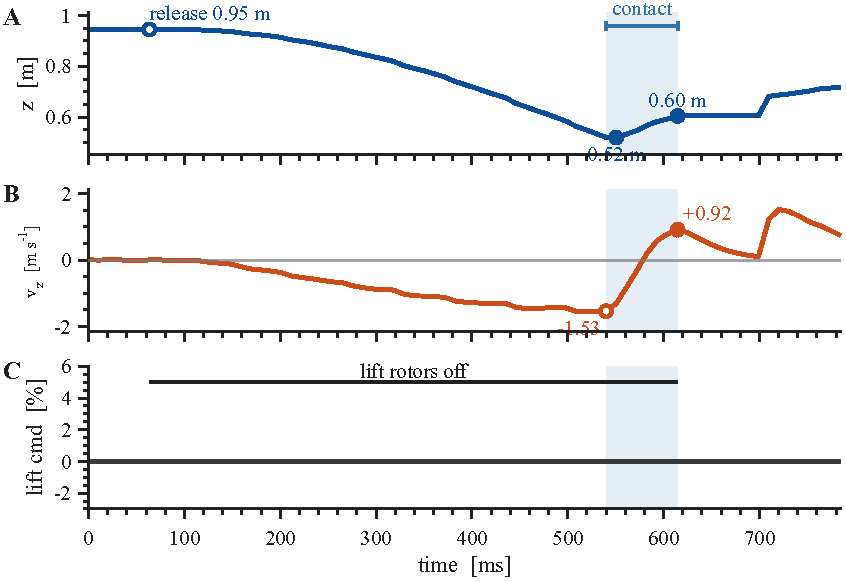
\includegraphics[width=0.72\linewidth]{Assets/ch5fig1_single_hop.pdf}
    \caption{A single water-skipping hop, with the lift rotors commanded
    off throughout.  \textbf{(A)}~Height.  The vehicle is released from a
    hover at $0.94\;\mathrm{m}$, descends to $0.52\;\mathrm{m}$, and has
    recovered to $0.61\;\mathrm{m}$ by the time the foils leave the water.
    \textbf{(B)}~Vertical velocity.  The shaded band marks the water
    contact, bounded by the two turning points of the velocity trace: entry
    at $-1.55\;\mathrm{m\,s^{-1}}$, where the descent stops steepening, and
    exit at $+0.92\;\mathrm{m\,s^{-1}}$, where the water ceases to add
    upward speed.  \textbf{(C)}~Commanded lift thrust, as a percentage of
    full scale.  The command is cut from its hover value to zero before the
    descent and remains there through the contact and ejection; the bar
    marks the unpowered interval.  Control is restored shortly before the
    apex at a thrust-to-weight ratio below $0.35$, which cannot support the
    vehicle and is omitted from the trace for clarity.}
    \label{fig:hop_single}
\end{figure}